\documentclass[11pt,preprint, authoryear]{elsarticle}

\usepackage{lmodern}
%%%% My spacing
\usepackage{setspace}
\setstretch{1.2}
\DeclareMathSizes{12}{14}{10}{10}

% Wrap around which gives all figures included the [H] command, or places it "here". This can be tedious to code in Rmarkdown.
\usepackage{float}
\let\origfigure\figure
\let\endorigfigure\endfigure
\renewenvironment{figure}[1][2] {
    \expandafter\origfigure\expandafter[H]
} {
    \endorigfigure
}

\let\origtable\table
\let\endorigtable\endtable
\renewenvironment{table}[1][2] {
    \expandafter\origtable\expandafter[H]
} {
    \endorigtable
}


\usepackage{ifxetex,ifluatex}
\usepackage{fixltx2e} % provides \textsubscript
\ifnum 0\ifxetex 1\fi\ifluatex 1\fi=0 % if pdftex
  \usepackage[T1]{fontenc}
  \usepackage[utf8]{inputenc}
\else % if luatex or xelatex
  \ifxetex
    \usepackage{mathspec}
    \usepackage{xltxtra,xunicode}
  \else
    \usepackage{fontspec}
  \fi
  \defaultfontfeatures{Mapping=tex-text,Scale=MatchLowercase}
  \newcommand{\euro}{€}
\fi

\usepackage{amssymb, amsmath, amsthm, amsfonts}

\def\bibsection{\section*{References}} %%% Make "References" appear before bibliography


\usepackage[round]{natbib}

\usepackage{longtable}
\usepackage[margin=2.3cm,bottom=2cm,top=2.5cm, includefoot]{geometry}
\usepackage{fancyhdr}
\usepackage[bottom, hang, flushmargin]{footmisc}
\usepackage{graphicx}
\numberwithin{equation}{section}
\numberwithin{figure}{section}
\numberwithin{table}{section}
\setlength{\parindent}{0cm}
\setlength{\parskip}{1.3ex plus 0.5ex minus 0.3ex}
\usepackage{textcomp}
\renewcommand{\headrulewidth}{0.2pt}
\renewcommand{\footrulewidth}{0.3pt}

\usepackage{array}
\newcolumntype{x}[1]{>{\centering\arraybackslash\hspace{0pt}}p{#1}}

%%%%  Remove the "preprint submitted to" part. Don't worry about this either, it just looks better without it:
\makeatletter
\def\ps@pprintTitle{%
  \let\@oddhead\@empty
  \let\@evenhead\@empty
  \let\@oddfoot\@empty
  \let\@evenfoot\@oddfoot
}
\makeatother

 \def\tightlist{} % This allows for subbullets!

\usepackage{hyperref}
\hypersetup{breaklinks=true,
            bookmarks=true,
            colorlinks=true,
            citecolor=blue,
            urlcolor=blue,
            linkcolor=blue,
            pdfborder={0 0 0}}


% The following packages allow huxtable to work:
\usepackage{siunitx}
\usepackage{multirow}
\usepackage{hhline}
\usepackage{calc}
\usepackage{tabularx}
\usepackage{booktabs}
\usepackage{caption}


\newenvironment{columns}[1][]{}{}

\newenvironment{column}[1]{\begin{minipage}{#1}\ignorespaces}{%
\end{minipage}
\ifhmode\unskip\fi
\aftergroup\useignorespacesandallpars}

\def\useignorespacesandallpars#1\ignorespaces\fi{%
#1\fi\ignorespacesandallpars}

\makeatletter
\def\ignorespacesandallpars{%
  \@ifnextchar\par
    {\expandafter\ignorespacesandallpars\@gobble}%
    {}%
}
\makeatother

\newenvironment{CSLReferences}[2]{%
}

\urlstyle{same}  % don't use monospace font for urls
\setlength{\parindent}{0pt}
\setlength{\parskip}{6pt plus 2pt minus 1pt}
\setlength{\emergencystretch}{3em}  % prevent overfull lines
\setcounter{secnumdepth}{5}

%%% Use protect on footnotes to avoid problems with footnotes in titles
\let\rmarkdownfootnote\footnote%
\def\footnote{\protect\rmarkdownfootnote}
\IfFileExists{upquote.sty}{\usepackage{upquote}}{}

%%% Include extra packages specified by user
\usepackage{array}
\usepackage{caption}
\usepackage{graphicx}
\usepackage{siunitx}
\usepackage[normalem]{ulem}
\usepackage{colortbl}
\usepackage{multirow}
\usepackage{hhline}
\usepackage{calc}
\usepackage{tabularx}
\usepackage{threeparttable}
\usepackage{wrapfig}
\usepackage{adjustbox}
\usepackage{hyperref}

%%% Hard setting column skips for reports - this ensures greater consistency and control over the length settings in the document.
%% page layout
%% paragraphs
\setlength{\baselineskip}{12pt plus 0pt minus 0pt}
\setlength{\parskip}{12pt plus 0pt minus 0pt}
\setlength{\parindent}{0pt plus 0pt minus 0pt}
%% floats
\setlength{\floatsep}{12pt plus 0 pt minus 0pt}
\setlength{\textfloatsep}{20pt plus 0pt minus 0pt}
\setlength{\intextsep}{14pt plus 0pt minus 0pt}
\setlength{\dbltextfloatsep}{20pt plus 0pt minus 0pt}
\setlength{\dblfloatsep}{14pt plus 0pt minus 0pt}
%% maths
\setlength{\abovedisplayskip}{12pt plus 0pt minus 0pt}
\setlength{\belowdisplayskip}{12pt plus 0pt minus 0pt}
%% lists
\setlength{\topsep}{10pt plus 0pt minus 0pt}
\setlength{\partopsep}{3pt plus 0pt minus 0pt}
\setlength{\itemsep}{5pt plus 0pt minus 0pt}
\setlength{\labelsep}{8mm plus 0mm minus 0mm}
\setlength{\parsep}{\the\parskip}
\setlength{\listparindent}{\the\parindent}
%% verbatim
\setlength{\fboxsep}{5pt plus 0pt minus 0pt}



\begin{document}



\begin{frontmatter}  %

\title{Question 5: Googleplay}

% Set to FALSE if wanting to remove title (for submission)




\author[Add1]{Grace Grant}
\ead{21653488@sun.ac.za}





\address[Add1]{Stellenbosch University, Stellenbosch, South Africa}



\vspace{1cm}





\vspace{0.5cm}

\end{frontmatter}

\setcounter{footnote}{0}



%________________________
% Header and Footers
%%%%%%%%%%%%%%%%%%%%%%%%%%%%%%%%%
\pagestyle{fancy}
\chead{}
\rhead{}
\lfoot{}
\rfoot{\footnotesize Page \thepage}
\lhead{}
%\rfoot{\footnotesize Page \thepage } % "e.g. Page 2"
\cfoot{}

%\setlength\headheight{30pt}
%%%%%%%%%%%%%%%%%%%%%%%%%%%%%%%%%
%________________________

\headsep 35pt % So that header does not go over title




\hypertarget{app-size-and-ratings-linked-to-number-of-installs}{%
\section{App size and ratings linked to number of
installs}\label{app-size-and-ratings-linked-to-number-of-installs}}

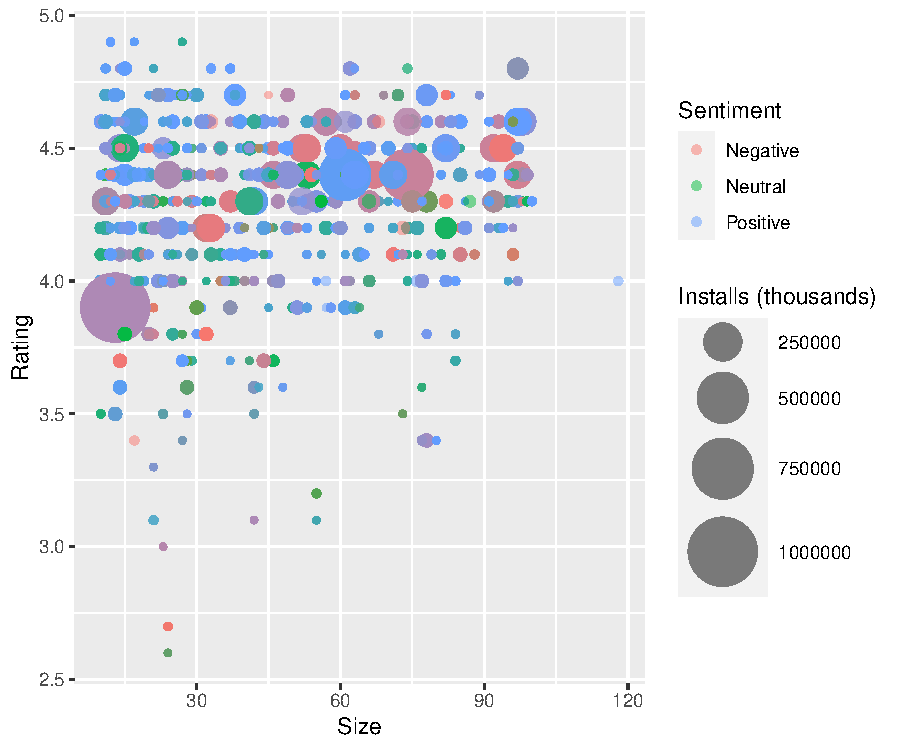
\includegraphics{Question-5-again_files/figure-latex/unnamed-chunk-1-1.pdf}

The graph provided above gives an indication of the link between the
size of the app and its rating, with most apps having ratings above 4
and sizes below 100M. I would, therefore, suggest an app with a size
below 100M. The graph also shows that, while most apps are linked to
positive reviewer sentiment, there does not seem to be a link between
reviewer sentiment and the number of installations. This can show that,
even though it is important to listen to what reviews have to say, this
does not necessarily correlate with how many people choose to install an
app. If profitability is linked to the number of installations, it would
be a better idea to focus on the app rating and keeping those numbers
high while also ensuring that apps are not too big in size.

\hypertarget{app-ratings-and-categories}{%
\section{App ratings and categories}\label{app-ratings-and-categories}}

 
  \providecommand{\huxb}[2]{\arrayrulecolor[RGB]{#1}\global\arrayrulewidth=#2pt}
  \providecommand{\huxvb}[2]{\color[RGB]{#1}\vrule width #2pt}
  \providecommand{\huxtpad}[1]{\rule{0pt}{#1}}
  \providecommand{\huxbpad}[1]{\rule[-#1]{0pt}{#1}}

\begin{table}[ht]
\begin{centerbox}
\begin{threeparttable}
 \label{tab:unnamed-chunk-2}
\setlength{\tabcolsep}{0pt}
\begin{tabular}{l l l}


\hhline{>{\huxb{0, 0, 0}{1}}->{\huxb{0, 0, 0}{1}}->{\huxb{0, 0, 0}{1}}-}
\arrayrulecolor{black}

\multicolumn{1}{!{\huxvb{0, 0, 0}{1}}l!{\huxvb{0, 0, 0}{1}}}{\huxtpad{6pt + 1em}\raggedright \hspace{6pt} {\fontsize{10pt}{12pt}\selectfont App} \hspace{6pt}\huxbpad{6pt}} &
\multicolumn{1}{l!{\huxvb{0, 0, 0}{1}}}{\huxtpad{6pt + 1em}\raggedright \hspace{6pt} {\fontsize{10pt}{12pt}\selectfont Category} \hspace{6pt}\huxbpad{6pt}} &
\multicolumn{1}{r!{\huxvb{0, 0, 0}{1}}}{\huxtpad{6pt + 1em}\raggedleft \hspace{6pt} {\fontsize{10pt}{12pt}\selectfont Rating} \hspace{6pt}\huxbpad{6pt}} \tabularnewline[-0.5pt]


\hhline{>{\huxb{0, 0, 0}{1}}->{\huxb{0, 0, 0}{1}}->{\huxb{0, 0, 0}{1}}-}
\arrayrulecolor{black}

\multicolumn{1}{!{\huxvb{0, 0, 0}{1}}l!{\huxvb{0, 0, 0}{1}}}{\huxtpad{6pt + 1em}\raggedright \hspace{6pt} {\fontsize{10pt}{12pt}\selectfont CDL Practice Test 2018 Edition} \hspace{6pt}\huxbpad{6pt}} &
\multicolumn{1}{l!{\huxvb{0, 0, 0}{1}}}{\huxtpad{6pt + 1em}\raggedright \hspace{6pt} {\fontsize{10pt}{12pt}\selectfont AUTO\_AND\_VEHICLES} \hspace{6pt}\huxbpad{6pt}} &
\multicolumn{1}{r!{\huxvb{0, 0, 0}{1}}}{\huxtpad{6pt + 1em}\raggedleft \hspace{6pt} {\fontsize{10pt}{12pt}\selectfont 4.9} \hspace{6pt}\huxbpad{6pt}} \tabularnewline[-0.5pt]


\hhline{>{\huxb{0, 0, 0}{1}}->{\huxb{0, 0, 0}{1}}->{\huxb{0, 0, 0}{1}}-}
\arrayrulecolor{black}

\multicolumn{1}{!{\huxvb{0, 0, 0}{1}}l!{\huxvb{0, 0, 0}{1}}}{\huxtpad{6pt + 1em}\raggedright \hspace{6pt} {\fontsize{10pt}{12pt}\selectfont DMV Permit Practice Test 2018 Edition} \hspace{6pt}\huxbpad{6pt}} &
\multicolumn{1}{l!{\huxvb{0, 0, 0}{1}}}{\huxtpad{6pt + 1em}\raggedright \hspace{6pt} {\fontsize{10pt}{12pt}\selectfont AUTO\_AND\_VEHICLES} \hspace{6pt}\huxbpad{6pt}} &
\multicolumn{1}{r!{\huxvb{0, 0, 0}{1}}}{\huxtpad{6pt + 1em}\raggedleft \hspace{6pt} {\fontsize{10pt}{12pt}\selectfont 4.9} \hspace{6pt}\huxbpad{6pt}} \tabularnewline[-0.5pt]


\hhline{>{\huxb{0, 0, 0}{1}}->{\huxb{0, 0, 0}{1}}->{\huxb{0, 0, 0}{1}}-}
\arrayrulecolor{black}

\multicolumn{1}{!{\huxvb{0, 0, 0}{1}}l!{\huxvb{0, 0, 0}{1}}}{\huxtpad{6pt + 1em}\raggedright \hspace{6pt} {\fontsize{10pt}{12pt}\selectfont Down Dog: Great Yoga Anywhere} \hspace{6pt}\huxbpad{6pt}} &
\multicolumn{1}{l!{\huxvb{0, 0, 0}{1}}}{\huxtpad{6pt + 1em}\raggedright \hspace{6pt} {\fontsize{10pt}{12pt}\selectfont HEALTH\_AND\_FITNESS} \hspace{6pt}\huxbpad{6pt}} &
\multicolumn{1}{r!{\huxvb{0, 0, 0}{1}}}{\huxtpad{6pt + 1em}\raggedleft \hspace{6pt} {\fontsize{10pt}{12pt}\selectfont 4.9} \hspace{6pt}\huxbpad{6pt}} \tabularnewline[-0.5pt]


\hhline{>{\huxb{0, 0, 0}{1}}->{\huxb{0, 0, 0}{1}}->{\huxb{0, 0, 0}{1}}-}
\arrayrulecolor{black}

\multicolumn{1}{!{\huxvb{0, 0, 0}{1}}l!{\huxvb{0, 0, 0}{1}}}{\huxtpad{6pt + 1em}\raggedright \hspace{6pt} {\fontsize{10pt}{12pt}\selectfont Amino: Communities and Chats} \hspace{6pt}\huxbpad{6pt}} &
\multicolumn{1}{l!{\huxvb{0, 0, 0}{1}}}{\huxtpad{6pt + 1em}\raggedright \hspace{6pt} {\fontsize{10pt}{12pt}\selectfont SOCIAL} \hspace{6pt}\huxbpad{6pt}} &
\multicolumn{1}{r!{\huxvb{0, 0, 0}{1}}}{\huxtpad{6pt + 1em}\raggedleft \hspace{6pt} {\fontsize{10pt}{12pt}\selectfont 4.8} \hspace{6pt}\huxbpad{6pt}} \tabularnewline[-0.5pt]


\hhline{>{\huxb{0, 0, 0}{1}}->{\huxb{0, 0, 0}{1}}->{\huxb{0, 0, 0}{1}}-}
\arrayrulecolor{black}

\multicolumn{1}{!{\huxvb{0, 0, 0}{1}}l!{\huxvb{0, 0, 0}{1}}}{\huxtpad{6pt + 1em}\raggedright \hspace{6pt} {\fontsize{10pt}{12pt}\selectfont Calculator with Percent (Free)} \hspace{6pt}\huxbpad{6pt}} &
\multicolumn{1}{l!{\huxvb{0, 0, 0}{1}}}{\huxtpad{6pt + 1em}\raggedright \hspace{6pt} {\fontsize{10pt}{12pt}\selectfont TOOLS} \hspace{6pt}\huxbpad{6pt}} &
\multicolumn{1}{r!{\huxvb{0, 0, 0}{1}}}{\huxtpad{6pt + 1em}\raggedleft \hspace{6pt} {\fontsize{10pt}{12pt}\selectfont 4.8} \hspace{6pt}\huxbpad{6pt}} \tabularnewline[-0.5pt]


\hhline{>{\huxb{0, 0, 0}{1}}->{\huxb{0, 0, 0}{1}}->{\huxb{0, 0, 0}{1}}-}
\arrayrulecolor{black}

\multicolumn{1}{!{\huxvb{0, 0, 0}{1}}l!{\huxvb{0, 0, 0}{1}}}{\huxtpad{6pt + 1em}\raggedright \hspace{6pt} {\fontsize{10pt}{12pt}\selectfont DU Recorder – Screen Recorder, Video Editor, Live} \hspace{6pt}\huxbpad{6pt}} &
\multicolumn{1}{l!{\huxvb{0, 0, 0}{1}}}{\huxtpad{6pt + 1em}\raggedright \hspace{6pt} {\fontsize{10pt}{12pt}\selectfont VIDEO\_PLAYERS} \hspace{6pt}\huxbpad{6pt}} &
\multicolumn{1}{r!{\huxvb{0, 0, 0}{1}}}{\huxtpad{6pt + 1em}\raggedleft \hspace{6pt} {\fontsize{10pt}{12pt}\selectfont 4.8} \hspace{6pt}\huxbpad{6pt}} \tabularnewline[-0.5pt]


\hhline{>{\huxb{0, 0, 0}{1}}->{\huxb{0, 0, 0}{1}}->{\huxb{0, 0, 0}{1}}-}
\arrayrulecolor{black}

\multicolumn{1}{!{\huxvb{0, 0, 0}{1}}l!{\huxvb{0, 0, 0}{1}}}{\huxtpad{6pt + 1em}\raggedright \hspace{6pt} {\fontsize{10pt}{12pt}\selectfont Even - organize your money, get paid early} \hspace{6pt}\huxbpad{6pt}} &
\multicolumn{1}{l!{\huxvb{0, 0, 0}{1}}}{\huxtpad{6pt + 1em}\raggedright \hspace{6pt} {\fontsize{10pt}{12pt}\selectfont FINANCE} \hspace{6pt}\huxbpad{6pt}} &
\multicolumn{1}{r!{\huxvb{0, 0, 0}{1}}}{\huxtpad{6pt + 1em}\raggedleft \hspace{6pt} {\fontsize{10pt}{12pt}\selectfont 4.8} \hspace{6pt}\huxbpad{6pt}} \tabularnewline[-0.5pt]


\hhline{>{\huxb{0, 0, 0}{1}}->{\huxb{0, 0, 0}{1}}->{\huxb{0, 0, 0}{1}}-}
\arrayrulecolor{black}

\multicolumn{1}{!{\huxvb{0, 0, 0}{1}}l!{\huxvb{0, 0, 0}{1}}}{\huxtpad{6pt + 1em}\raggedright \hspace{6pt} {\fontsize{10pt}{12pt}\selectfont Find a Way: Addictive Puzzle} \hspace{6pt}\huxbpad{6pt}} &
\multicolumn{1}{l!{\huxvb{0, 0, 0}{1}}}{\huxtpad{6pt + 1em}\raggedright \hspace{6pt} {\fontsize{10pt}{12pt}\selectfont FAMILY} \hspace{6pt}\huxbpad{6pt}} &
\multicolumn{1}{r!{\huxvb{0, 0, 0}{1}}}{\huxtpad{6pt + 1em}\raggedleft \hspace{6pt} {\fontsize{10pt}{12pt}\selectfont 4.8} \hspace{6pt}\huxbpad{6pt}} \tabularnewline[-0.5pt]


\hhline{>{\huxb{0, 0, 0}{1}}->{\huxb{0, 0, 0}{1}}->{\huxb{0, 0, 0}{1}}-}
\arrayrulecolor{black}

\multicolumn{1}{!{\huxvb{0, 0, 0}{1}}l!{\huxvb{0, 0, 0}{1}}}{\huxtpad{6pt + 1em}\raggedright \hspace{6pt} {\fontsize{10pt}{12pt}\selectfont FreePrints – Free Photos Delivered} \hspace{6pt}\huxbpad{6pt}} &
\multicolumn{1}{l!{\huxvb{0, 0, 0}{1}}}{\huxtpad{6pt + 1em}\raggedright \hspace{6pt} {\fontsize{10pt}{12pt}\selectfont PHOTOGRAPHY} \hspace{6pt}\huxbpad{6pt}} &
\multicolumn{1}{r!{\huxvb{0, 0, 0}{1}}}{\huxtpad{6pt + 1em}\raggedleft \hspace{6pt} {\fontsize{10pt}{12pt}\selectfont 4.8} \hspace{6pt}\huxbpad{6pt}} \tabularnewline[-0.5pt]


\hhline{>{\huxb{0, 0, 0}{1}}->{\huxb{0, 0, 0}{1}}->{\huxb{0, 0, 0}{1}}-}
\arrayrulecolor{black}

\multicolumn{1}{!{\huxvb{0, 0, 0}{1}}l!{\huxvb{0, 0, 0}{1}}}{\huxtpad{6pt + 1em}\raggedright \hspace{6pt} {\fontsize{10pt}{12pt}\selectfont Fuzzy Seasons: Animal Forest} \hspace{6pt}\huxbpad{6pt}} &
\multicolumn{1}{l!{\huxvb{0, 0, 0}{1}}}{\huxtpad{6pt + 1em}\raggedright \hspace{6pt} {\fontsize{10pt}{12pt}\selectfont FAMILY} \hspace{6pt}\huxbpad{6pt}} &
\multicolumn{1}{r!{\huxvb{0, 0, 0}{1}}}{\huxtpad{6pt + 1em}\raggedleft \hspace{6pt} {\fontsize{10pt}{12pt}\selectfont 4.8} \hspace{6pt}\huxbpad{6pt}} \tabularnewline[-0.5pt]


\hhline{>{\huxb{0, 0, 0}{1}}->{\huxb{0, 0, 0}{1}}->{\huxb{0, 0, 0}{1}}-}
\arrayrulecolor{black}
\end{tabular}
\end{threeparttable}\par\end{centerbox}

\end{table}
 

This table shows the categories that the top 10 highest rated apps fall
into. There are quite a variety of categories in the top 20 but many of
the categories are linked to ways that help people, whether this is with
health, navigation, mathematics or practising for a written driving
test. I would thus suggest creating an app that offers a helpful
service, maybe linked to the health and fitness category.

\bibliography{Tex/ref}





\end{document}
